\chapter{Design}

\section{Overview}
The algorithm that has produced as a part of this project has two main components: the first component calculates and finds blocks of code which match between two revisions of the code (i.e. between two commits), the second uses the matching blocks to calculate the code contributions for all of the users that contributed to a single file. The proposed algorithm's abstraction analyses the repository at the character level and has the properties discussed in Section 1.1, namely, awareness of code quality, and versatility to change. The way the project was approached was inspired by a study carried out to test and compare quality of open-source contributions on Wikipedia \citep{10.1145/1531674.1531682}. While this research project was looking into a single language of English and using a tokenisation approach, this project aims to be independent of programming languages. This property is more useful in a student group project environment. The approach proposed for this project (using character-level abstraction) has two main reasons and advantages: the algorithm does not require a tokenisation algorithm for each individual programming language and it also removes subjectiveness for certain tokens or certain sections of code that are recognised as more important (for example, is the main function that is only called once more important than a class method that is called multiple times throughout the code?). Rather, the algorithm assumes and evaluates importance from users' evaluation via modification of the existing code. By definition, any code or characters that has changes made to it by other contributors will persist and is regarded as good quality code.

Calculations between commits are made at a character-level abstraction and are implemented using the concept of longest common subsequence \citep{wiki:lcs}, which is one of the basis of data comparison programs such as the \textit{diff} function (as discussed previously in Section 2.2). The algorithm implemented for the longest common subsequence was initially developed by John W. Ratciff and John A. Obershelp in 1983 and is sometimes referred to as Gestalt Pattern Matching \citep{wiki:gpm}. This algorithm was implemented from scratch in Ruby and was inspired by Python's \textit{difflib} library \citep{python_software_foundation_2021}. This implementation in Python had a class called \textit{SequenceMatcher}, which was the name given to their implementation of the Gestalt Pattern Matching algorithm. \textit{SequenceMatcher} also used an automatic junk management algorithm, which was not implemented in this project as the junk management is carried out a higher level of the algorithm. In this project's implementation of the Gestalt Pattern Matching algorithm, the output produced is a ratio of similarity between two strings \textit{a} and \textit{b} with a list of Match objects (i.e. $m = (a = 1, b = 2, size = 3)$) such that \textit{$m_a$} is the starting index of the matched subsequence in the string \textit{a}, \textit{$m_b$} is the starting index of the matched subsequence in the string \textit{b}, and \textit{$m_{size}$} is the length of the matched subsequence.

The Gestalt Pattern Matching algorithm is efficient when it comes to distinguishing any changes between strings (namely, additions, deletions and replacements). On the other hand, it lacks when it comes to detecting movements within a codebase. Movement events in a codebase, such as major refactoring, are considered by the algorithm as brand new code. Below is an example to demonstrate this behaviour by the Gestalt algorithm:
\begin{figure}
    \centering
    \begin{minted}[
    frame=lines,
    framesep=2mm,
    baselinestretch=1.2,
    bgcolor=black,
    linenos
    ]{cpp}
    infostream<<"Ban:"<<m_banfilepath;
    std::ofstream os(m_banfilepath);
    if(os.good == false) {
        infostream<<"Ban failed:"<<m_banfilepath;
        throw SerializationError("BanM::load()");
    }
    for(std::map<std::string, std::string>
        ::iterator
            i = m_ips.begin();
            i != m_ips.end(); i++)
    {
        os<<i->first<<"2"<<i->second<<"/n";
    }
    m_modified = false;
    \end{minted}
    \caption{Example code written in C++ \citep{ahola_2018}}
    \label{fig:1}
\end{figure}



Another contributor comes to edit the above code and creates a commit with the following revision (the changes have been highlighted in blue):
\begin{figure}
    \centering
    \setlength{\fboxsep}{1pt}
    \begin{minted}[
    frame=lines,
    framesep=2mm,
    baselinestretch=1.2,
    bgcolor=black,
    linenos,
    escapeinside=||
    ]{cpp}
    infostream<<"Ban:"<<m_banfilepath;
    std::o|\colorbox{blue}{string}|stream |\colorbox{blue}{s}|s(|\colorbox{blue}{std::ios\_base}|);
    for(std::map<std::string, std::string>
        ::iterator
            i = m_ips.begin();
            i != m_ips.end(); i++)
    {
        |\colorbox{blue}{s}|s << i->first << "2" <<i->second << "/n";
    }
    |\colorbox{blue}{if(!fs::WriteTo(m\_banfilepath, ss.str()))}|
    {
        infostream<<"Ban failed:"<<m_banfilepath;
        throw SerializationError("BanM::load()");
    }
    m_modified = false;
    \end{minted}
    \caption{Revision of code written in Figure 1 \citep{ahola_2018}}
    \label{fig:2}
\end{figure}

The revision by the user involves a refactor to change the boolean condition contained with the \textit{if} statement. Considering that the \textit{if} condition has been entirely reworked, the algorithm should decipher that that line is completely new. Some parts of the code have also been moved from below the \textit{if} statement to above it, while others have remained in place. There are also trivial changes in whitespace around line 8, which are not highlighted for this example.\\Gestalt's algorithm determines the following to be the changes made after processing all the subsequences:

\begin{figure}
    \centering
    \sethlcolor{blue}
    \begin{minted}[
    frame=lines,
    framesep=2mm,
    baselinestretch=1.2,
    bgcolor=black,
    linenos,
    escapeinside=||,
    highlightlines=3-9,
    highlightcolor=blue
    ]{cpp}
    infostream<<"Ban:"<<m_banfilepath;
    std::o|\hl{string}|stream |\hl{ss(std::}|ios|\hl{\_base);}|
    for(std::map<std::string,std::string>
        ::iterator
            i = m_ips.begin();
            i != m_ips.end(); i++)
    {
        ss << i->first << "2" << i->second << "/n";
    }
    |\hl{if(!fs::WriteTo}(m\_banfilepath, \hl{ss}.str())\hl{)}|
    {
        infostream<<"Ban failed:"<<m_banfilepath;
        throw SerializationError("BanM::load()");
    }
    m_modified = false;
    \end{minted}
    \caption{Revision in \ref{fig:2} as analysed by the Gestalt algorithm \citep{ahola_2018}}
    \label{fig:3}
\end{figure}

This limitation to the algorithm is persistent throughout other diff software as their purpose is to display and calculate how one string can be converted to another and not to show who made the changes. This limitation is emulated in a similar manner in the git-blame tool. However, the git-author tool has a solution to this limitation by using a more powerful diff tool (ldiff) that is able to detect line movements \citep{6676896}. The first part of the algorithm (Algorithm 1) proposed in this project tracks line movements as well as character additions, deletions and replacements. This is done using a similar approach to ldiff \citep{5070564}. This part returns an array of Match objects representing matching characters between two strings.

\begin{algorithm}[htp]
\SetKwFor{For}{for}{do}{{end for} for}
\SetKwIF{If}{ElseIf}{Else}{if}{then}{else if}{else}{{end if}}
\SetAlgoLined\DontPrintSemicolon
\SetKwFunction{proc}{CalculateLineChanges}
\SetKwProg{myproc}{procedure}{}{{end procedure}}
\myproc{\proc{\textit{old}, \textit{new}, \textit{threshold} = 0.6}} {
  $A \longleftarrow$ list of lines in \textit{old}\;
  $B \longleftarrow$ list of lines in \textit{new}\;
  $pos \longleftarrow 0$\;
  \For{a in range(0, length(\textit{A}))}{
    First(A).append(\textit{pos})\;
    \textit{pos} \longleftarrow $\textit{pos} + length(A_a)$\;
  }
  $\textit{pos} \longleftarrow 0$\;
  \For{\textit{b} in range(0, length(B))}{
    First(B).append(pos)\;
    pos \longleftarrow $pos + length(B_b)$\;
  }
  $diffs \longleftarrow []$\;
  $ylist \longleftarrow range(0, length(B))$\;
  \For{a in range(0, length(A))}{
    \For{b in range(0,length(ylist))}{
      $ratio \longleftarrow Gestalt (A_a, B_{ylist_b})$ similarity ratio\;
      $matchchars \longleftarrow {Gestalt (A_a, B_{ylist_b})}$\;
      $diffs_{a,b}$ \longleftarrow (a, $ylist_b$, ratio, matchchars)\;
      \If{$ratio = 1$}{
        del($ylist_b$)\;
        Skip to $a + 1$\;
      }
    }
  }
  $toDelete \longleftarrow 0$\;
  \While{found = True}{
    $found \longleftarrow False$\;
    $max \longleftarrow (0,0,0,0,0)$\;
    \For{a in range(0, length(diffs))}{
      \For{b in range(0, length($diffs_a$))}{
        \lIf{$diffs_{a,b_1}$ = delete}{
          $diffs_{a,b}$ = (0, 0, 0, 0)
        }
        \lElseIf{$diffs_{a,b_2} > mt$ and $max_2 < diffs_{a,b_2}$}{
          max \longleftarrow ($diffs_{a,b_0}$, $diffs_{a,b_1}$, $diffs_{a,b_2}$, $diffs_{a,b_3}$, a)
        }
      }
    }
    \If{$max_2 = 0$}{
      $found = True$\;
      \For{m in $max_3$}{
        matches.append(($m_0 + A_{max_0}, m_1 + B_{max_1}, m_2$))
      }
      delete $diffs_{max_4}$\;
      delete \longleftarrow $max_1$\;
    }
  }
  \Return{matches} 
}
\caption{Calculate line changes}
\end{algorithm}
\newpage
The algorithm starts by splitting two different revisions of a block of text (\textit{old}, \textit{new}) into arrays of strings (\textit{A}, \textit{B}). This split happens using built-in string functions that divides lines on new line characters while also preserving the new line characters in each line. The function then calculates and distinguishes the starting characters of these lines (First(A), First(B)). For each line in the first array \textit{A}, the algorithm would compare them to the second array \textit{B} and the results that were found were stored into a tuple of 4 objects. These include the lines numbers of the compared lines (in both A and B), the similarity score/ratio given between the two selections of text, and the Match objects for the matched lines. As shown in Algorithm 1, the only time when the Gestalt algorithm is run is in lines 18 and 19. However, these lines depict one execution of the Gestalt algorithm, so for clarity this has been split into two lines. 

One place where an optimisation was made to stop comparisons of previously identified lines in A and B using a dynamic list named \textit{ylist}. This list was reduced at run-time, limiting the number of iterations in a double \textit{for} loop in lines 16-26. This optimisation improves the algorithm's best-case time complexity from $\Omega(n*m)$ to simply $\Omega(n)$. However, for the algorithm to be in the best case, the number of identical lines found between the \textit{n} lines in \textit{A} and the \textit{m} lines in \textit{B}. Omitting avoidable iterations of the algorithm improves the running speed of the algorithm by a great factor, considering the Gestalt algorithm has a worst-case time complexity of $O(n^2)$. This optimisation works by deleting lines that have been compared to other lines in the past and does not delete lines that are determined to be identical. To complete the latter, the \textit{diffs} array would require a double iteration loop to access the $4^{th}$ element with all the Match objects. Alternatively, utilising a temporary, auxiliary variable (\textit{delete}) is the method responsible for deleting these lines.

Continuing, the algorithm loops through all the comparisons that produce a similarity score that is greater than the minimum change threshold \citep{10.1007/s10664-017-9575-4} where the threshold is defined as follows: 
$threshold \in \mathbb{R} \mid 0 < threshold \leq 1$. This \textit{threshold} is used in defining what lines are determined to be brand new additions. The objective of this parameter is to distinguish lines as changes to existing lines or brand new lines. An example where this threshold can be applied is looking at two strings ``x = x + 1" and ``x += 1". In this example, the similarity score is 0.66. If the threshold is considered to equal to 0.6 (like provided in Algorithm 1), the algorithm determines the two strings to be similar and in turn calculates the parts of the initial string that were changed using the Match objects returned by the Gestalt algorithm. On the other hand, when the similarity score is lower than the \textit{threshold}, the algorithm marks the line as new code. The reason for including this \textit{threshold} is to differentiate line movements from large additions supplemented with large removals. Another example to illustrate this necessity involves the two strings (seen at the start of chapter 4) ``\texttt{std::ofstream os(m\_banfilepath.c\_str());}" and ``\texttt{if(!fs:: safeWrite ToFile (m\_banfilepath, ss.str()))\{}" \citep{10.1007/s10664-017-9575-4}. As can be seen, there are a lot of overlapping characters between the two strings. However, the functionality of two strings is very different. In this case, one contributor may have completely removed the original line and written a new line of code. For these situations, the \textit{threshold} works to determine line movement within the code. The parameter protects any characters to be counted as the same as the previous revision when the new revision has had significant changes. 

The value of the \textit{threshold} is a very key part of the algorithm but can cause deviation in the results depending on the programming language of the files and repository. This is due to a difference between the average number of characters in each line in each programming language. This also means that rounding can become a problem when it comes to the \textit{threshold}. For example, if the \textit{threshold} = 0.6 and the number of characters in each line is 3, the result would be $\frac{\left \lfloor{0.6 * 3}\right \rceil}{3} = 0.667$. That causes the results to have an error of 3.4\% due to rounding for a discrete set of character lengths. The maximum error for the threshold in the algorithm can be calculated using this claim:\\
\newline
\textit{Claim 1} Let \textit{n} $\in \mathbb{Z}^+ | n > 0$ be the number of characters in a line and \textit{threshold} $\in \mathbb{R} | 0 < threshold \leq 1$ be the minimum threshold. Then the absolute maximum distortion to \textit{threshold} is $\abs{d_{max}} = \frac{1}{2n}$.\\

The proof of this claim can be found in the Appendix. Based on Claim 1 and Appendix 1, the absolute maximum difference $\abs{d_{max}}$ for $n = 1$ is equal to 50\%. This rounding error gets smaller when \textit{n} is increased. To demonstrate this practically and show the application of the rounding effect in regards to programming languages, the line length of common algorithms can be analysed to estimate a value for the average error that will given to the \textit{threshold}. Examples of these can be found on programming chrestomathy (a collection of solutions to problems in as many programming languages as possible) such as Rosetta Code. For this project, the bubble sort algorithm was analysed \citep{rosetta_code_2021}. For this algorithm, the average line character length is:
\begin{itemize}
    \item \textbf{C++}: 27 
    \item \textbf{LISP}: 33 
    \item \textbf{Erlang}: 19 
    \item \textbf{Go}: 20 
    \item \textbf{Java}: 23 
    \item \textbf{Perl}: 23 
    \item \textbf{Python}: 38 
    \item \textbf{Ruby}: 22 
    \item \textbf{C\#}: 27 
\end{itemize}
Using this information, an estimate for most common programming languages would be $n \geq 19$. Applying this to claim 1, the expected error would be $\pm 2.6\%$. This makes the error small enough for it to be ignored but significant enough to consider when select a value for the \textit{threshold}. 

After the most substantial Match object is distinguished from all the other entries in the two dimensional array \textit{diff}, there is a decision point which will help distinguish if a line is new or old. If the line is considered by the threshold to be similar enough to the previous revisions, the lines that have been matched together are appended to an array. The lines that have been matched are zeroed (instead of being deleted to preserve the array size) following this from the \textit{diff} array in line 34. The while loop from line 24 ends when all the Match objects above the threshold have been iterated over and returns an array of all the matching lines.

Running the first part of the algorithm on the previous example used for the Gestalt pattern matching algorithm in Figure 1 reveals the changes as displayed below:
\sethlcolor{blue}
\begin{figure}
    \centering
    \begin{minted}[
    frame=lines,
    framesep=2mm,
    baselinestretch=1.2,
    bgcolor=black,
    linenos,
    escapeinside=||,
    highlightlines=10,
    highlightcolor=blue
    ]{cpp}
    infostream<<"Ban:"<<m_banfilepath;
    std::|\hl{ostring}|stream |\hl{ss(std::i}|os_ba|\hl{s}|e);
    for(std::map<std::string,std::string>
        ::iterator
            i = m_ips.begin();
            i != m_ips.end(); i++)
    {
        |\hl{s}|s << i->first << "2" << i->second << "/n";
    }
    if(!fs::WriteTo(m_banfilepath, ss.str()))
    {
        infostream<<"Ban failed:"<<m_banfilepath;
        throw SerializationError("BanM::load()");
    }
    m_modified = false;
    \end{minted}
    \caption{Diff produced by Algorithm 1 when applied to revision of \ref{fig:1} \citep{ahola_2018}}
    \label{fig:4}
\end{figure}

Comparing the diff produced to the diff produced in Figure 2 that showed the actual differences in the file. To produce these results, a \textit{threshold} of 0.6 was used. A change in the \textit{threshold} can very easily change the result of this diff considerably. Larger values of the \textit{threshold} will result in a lot less lines being deemed similar as the evaluation of similarity is much more stern. This will bring about a higher likelihood that the algorithm analyzes the correct lines of code that look nearly indistinguishable. In any case, this causes the algorithm to also fail to identify line changes for lines that are under 60\% similarity. For the example described above, a \textit{threshold} of 0.7 would have caused line 2 to be distinguished as brand new line addition, which may seem valid as it has been reworked significantly.

The second part of the algorithm uses the previously described Algorithm 1 to fully implement code ownership. This is done as follows:

Let a file \textit{f} that has \textit{M} number of revisions/commits be represented as a list $R = \{ r_1, r_2, ..., r_m \}$. Each revision $r_i \in R$ contains a list of size $y$ that contains sentences split into characters $C = \{c_1, c_2, ..., c_y\}$ which represents the codebase of \textit{f}. Each $r_i$ is made by a different user $u_i$ from a list of contributors $U = \{u_1, u_2, ..., u_n\}$. 

The second part of the algorithm that attributes the character changes in \textit{f} for all the contributors in \textit{U} can be seen in Algorithm 2.

\begin{algorithm}[ht]
\SetKwFor{For}{for}{do}{{end for} for}
\SetKwIF{If}{ElseIf}{Else}{if}{then}{else if}{else}{{end if}}
\SetAlgoLined\DontPrintSemicolon
\SetKwFunction{proc}{CalculateContributions}
\SetKwProg{myproc}{procedure}{}{{end procedure}}
\myproc{\proc{R, base = 10, threshold = 0.6}}{
    $M \longleftarrow length(R)$\;
    \For{i in range(1,M)}{
        \uIf{i = 1}{
            $y \longleftarrow length(r_i)$\;
            $Y \longleftarrow $[i for y in range(0, y)]\;
        }
        \Else{
            $matches \longleftarrow CalculateLineChanges(r_{i-1}, r_i, threshold)$\;
            Sort \textit{matches} using $matches_{m, 1}$\;
            $pointer \longleftarrow 0$\;
            $Ynew \longleftarrow [\;]$\;
            \For{m in matches}{
                \If{$m_1 \neq pointer$}{
                    \For{range(0, $m_1 - pointer$)}{
                        $Ynew.append(i)$\;
                    }
                    $pointer \longleftarrow pointer + (m_1 - pointer)$\;
                }
                \For{x in range(0, $m_2$)}{
                    $Ynew$.append($Y_{m_0+x}$)\;
                }
            }
            \If{length($r_i$) $>$ length($Ynew$)}{
                \For{range(0, length($r_i$)) - length($Ynew$)}{
                    $Ynew$.append(i)\;
                }
            }
            $Y \longleftarrow Ynew$\;
        }
    }
    \For{$i$ in range(0, length($Y$))}{
        $score_i \longleftarrow M - Y_i + 1$\;
        $Persistence_{ruY_i} \longleftarrow Persistence_{ruY_i} + score_i$\;
        $NumOfChars_{ruy_i} \longleftarrow NumOfChars_{ruy_i} + 1$
    }
    \For{$i$ in range(1, length($Persistence$)}{
        $Persistence_i \longleftarrow log_{base}(Persistence_i)$
    }
    \Return{$[Persistence, NumOfChars]$}
}
\caption{Calculate contributions for each user to a file}
\end{algorithm}

The way this part of the algorithm works is it calculates the persistence scores using the character-level revision history produced by the first half in Algorithm 1. The array $Y$ is used as a commit attribution record for each $f$. When commits are processed with characters being added, removed and replaced, the array $Y$ is changed to reflect where the new lines of code came from. This is done by adding the current commit number $i$ to the array. An example of how this works follows:
If a user $u_1$ adds the following characters ``wxyz" to the code in the first commit $r_1$, $Y = (1,1,1,1)$. This code is changed in the following commit $r_2$ to ``waaz" made by a second user $u_2$. This makes the array $Y = (1,2,2,1)$. The reason the array $Y$ stores these commit numbers is to allow the code to be attributed to the user that made each revision using the $ru$ dictionary, which relates each user key to a revision value. This process can be seen in a larger visual example in \ref{fig:5}.
\begin{figure}[h]
    \centering
    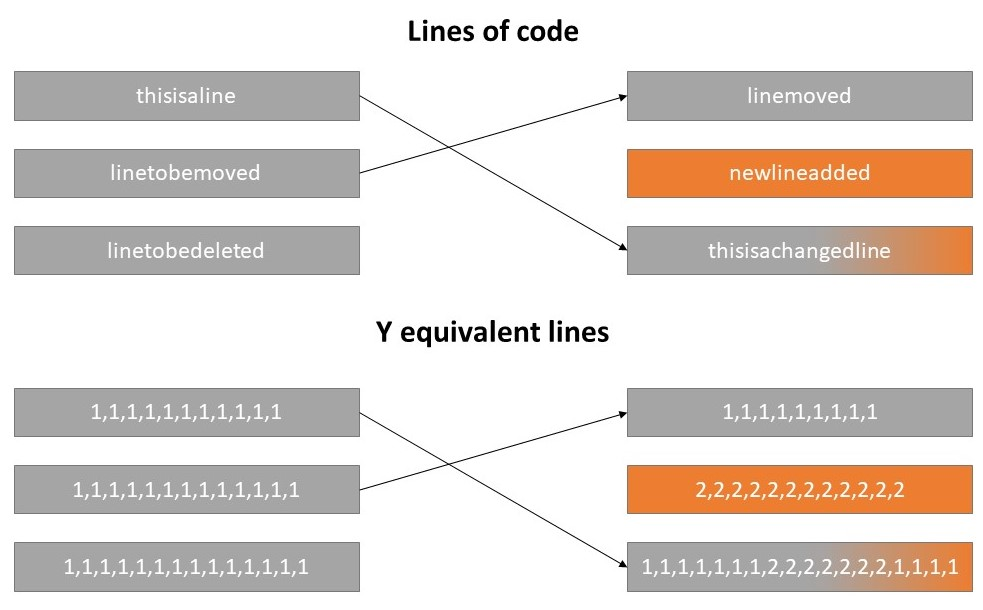
\includegraphics[scale=0.5]{images/tracking_changes.jpg}
    \caption{Changes between two commits at character level}
    \label{fig:5}
\end{figure}

The $score$ variable is used to hold the persistence score for each character and it indicates the quality of the code. This $score$ is only calculated after the final commit has been processed by the algorithm. This $score$ is calculated in line 35 and it practically inverses the results of the $Y$ array. The $score$ for each user is then finally processed by a log function, which counteracts the results produced by high volume and high traffic files that receive the majority of the commits. The $base$ of the log function can be modified to control the high volume of commits from users that write the bulk of the codebase at the start of a project. This procedure can be seen in Figure \ref{fig:6}. 
\begin{figure}[ht]
    \centering
    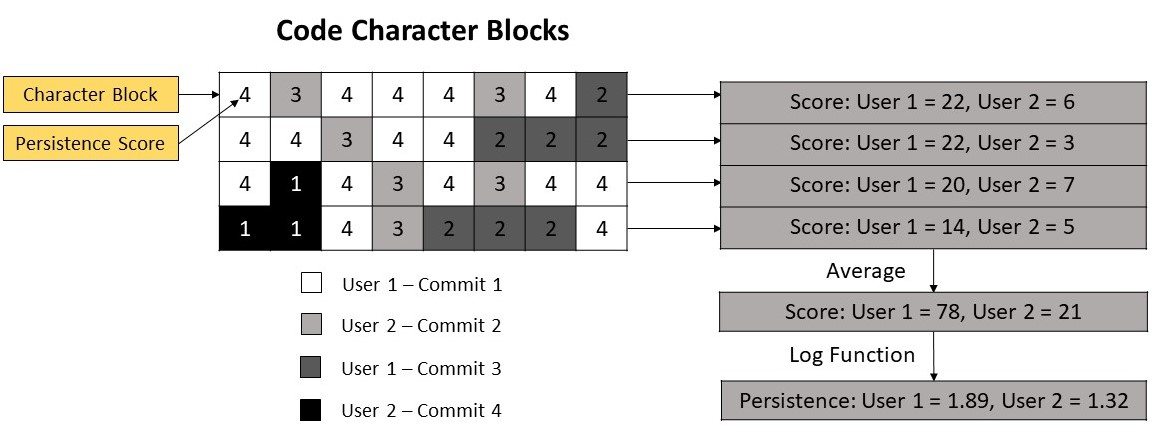
\includegraphics[scale=0.5]{images/persistence_calc.jpg}
    \caption{Visualisation of persistence calculation}
    \label{fig:6}
\end{figure}

In Figure \ref{fig:6}, User 1's contribution in terms of a percentage is $\frac{1.89}{(1.89+1.32)} \approx 59\%$. Analysing the same example using the methods discussed in Section 2.2, the $Chars$ measure that uses the character count gives a percentage of around 72\%. Using the $Commits$ measure, the percentage for User 1 is 50\%. $LOC$ and \textit{git-author} give results of 100\% and around 72\% respectively. The measures that use lower levels of abstraction give more accurate estimation but both $Chars$ and \textit{git-author} do not utilise the age of each character and just count each character as 1. For this project, the purpose is to give older character changes with greater value as this is definition of code quality as defined previously. User 1 has written the majority of the code. However, User 2 made changes in the $2^{nd}$ commit that have survived and have caused them to be labelled as important. 